En este primer capítulo de esta memoria se comentaran la motivación, los objetivos de la aplicación y la estructura de esta memoria. 
\section{Motivación}
Dado el creciente uso de los dispositivos móviles en los deportes al aire libre, como en caza y pesca, se aprecia una creciente demanda de aplicaciones que permitan el registro de estas actividades.\\
Por otro lado, la seguridad en estas actividades es un dato a tener en cuenta. Durante las jornadas de caza los cazadores caminan por el monte en grupos, esto puede producir que en determinados momentos un cazador no conozca la situación de su compañero.
Esta aplicación permitiría conocer la ubicación de cada cazador en todo momento pudiendo minimizar accidentes por disparos fortuitos. Las jornadas de pesca en ocasiones  se realizan desde acantilados o lugares muy lejos de carreteras, esto lleva a que si tenemos una pequeña lesión indicar nuestra ubicación a nuestros compañeros sea de gran ayuda.

Según datos del Consejo superior de deportes en España en el año 2016 se tramitaron 343.130 licencias federativas de caza y 54.992 licencias de pesca. Cabe destacar que existen tanto cazadores como pescadores que realizan sus actividades sin tener que estar federados, por lo que el número de licencias federativas aumentaría.





Por todo esto se propone este Trabajo de Fin de Grado.
El objetivo de este proyecto será diseñar y construir una herramienta que permita gestionar las actividades a campo abierto como
caza y pesca, permitiendo mediante geolocalización guardar los puntos de interés, las rutas seguidas,
llevar control de los usuarios presentes, guardar información de los éxitos de las jornadas y poder realizar jornadas de caza y pesca con un seguimiento  total de nuestros compañeros.


\section{Objetivos}
El objetivo es desarrollar una aplicación móvil en Android que permita al usuario realizar un seguimiento de sus jornadas tanto de caza como de pesca  y que le permita guardar sus puntos destacadas para poder visitarlos en otras ocasiones. Sin olvidar que el poder monitorizar la jornadas conjuntamente siempre es un punto a favor para seguridad de los participantes en estas actividades.\\ Los principales objetivos serán:

\begin{itemize}
\item Registro de usuarios y adición de amigos a usuario.
\item El usuario podrá conocer su ubicación en tiempo real en un mapa.
\item El usuario podrá comenzar y parar una jornada.
\item El usuario podrá visualizar la ruta seguida durante la jornada.
\item Administrar puntos clave para el usuario.
\item Clasificación de los puntos de interés según su tipología.
\item Visualizar dichos puntos en un mapa.
\item Gestionar grupos de usuarios participantes en la jornada y poder ver su ubicación en tiempo
real.

\end{itemize}


\section{Estructura de la memoria}
La memoria del presente proyecto está estructurada del siguiente modo:

\begin{itemize}
\item \textbf{Introducción} Contextualiza el proyecto, introduce el tema a tratar y detalla los objetivos del mismo desde un punto de vista global.
 También comenta la estructura de la memoria.

\item \textbf{Tecnología} Describe y justifica las principales tecnologías empleadas para desarrollar el proyecto.



\item \textbf{Proceso de ingeniería} Detallamos el proceso de ingeniería: la metodología empleada,como funcionada, la adaptación de la misma y los participantes.


\item \textbf{Análisis} Comentamos las funcionalidades de la aplicación, comentando más detenidamente los casos de uso y requisitos. 
\item \textbf{Seguimiento} Comentamos por las fases que pasa el proyecto usando la metodología Scrum.
\item \textbf{Diseño} Describimos la arquitectura del proyecto.
\item \textbf{Implementación} Describiremos aspectos concretos destacados y las pruebas realizadas.





\item \textbf{Conclusiones y trabajo futuro}
Comentamos el producto obtenido y futuros cambios que se podrían realizar.



\end{itemize}

\section{Estudio de mercado}
\subsection{iHunt Journal}

iHunt Journal es una aplicación de software de cacería que presenta las siguientes características: 
\begin{itemize}
\item Ver puntos en el mapa, figura \ref{fig:iHunt1}
\item Guardar puntos en un mapa,figura \ref{fig:iHunt2}
\item Puede grabar sus búsquedas.
\item Graba  estadísticas.
\item Permite planificar las próximas cacerías según meteorología, figura \ref{fig:iHunt3}.
\item Puede grabar sus trofeos figura \ref{fig:iHunt4}.

\end{itemize}

\begin{figure}[htbp]
\begin{minipage}[b]{0.5\linewidth} %Una minipágina que cubre la mitad de la página
\centering
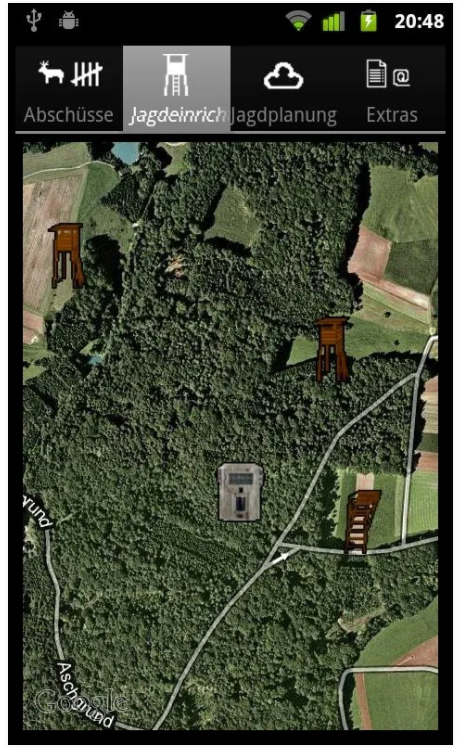
\includegraphics[width=6cm]{iHunt1.png}
\caption{ Visualizar mapa con iHunt}
\label{fig:iHunt1}
\end{minipage}
\hspace{0.5cm} % Si queremos tener un poco de espacio entre las dos figuras
\begin{minipage}[b]{0.5\linewidth}
\centering
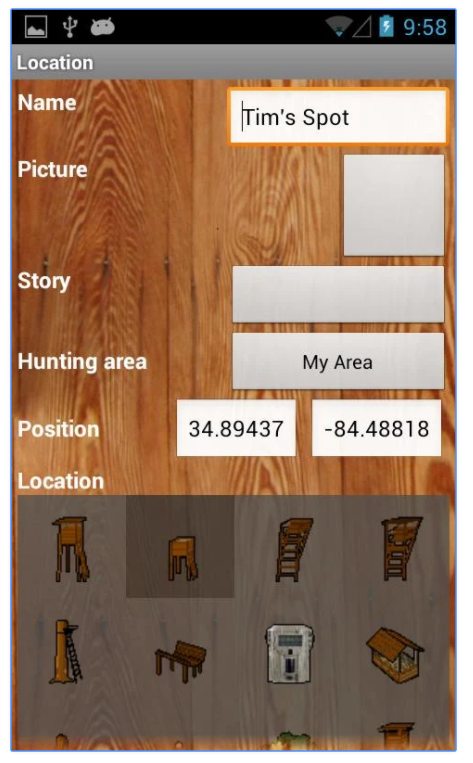
\includegraphics[width=6cm]{iHunt2.png}

\caption{Registro de un punto con iHunt}
\label{fig:iHunt2}
\end{minipage}
\begin{minipage}[b]{0.5\linewidth}
\centering
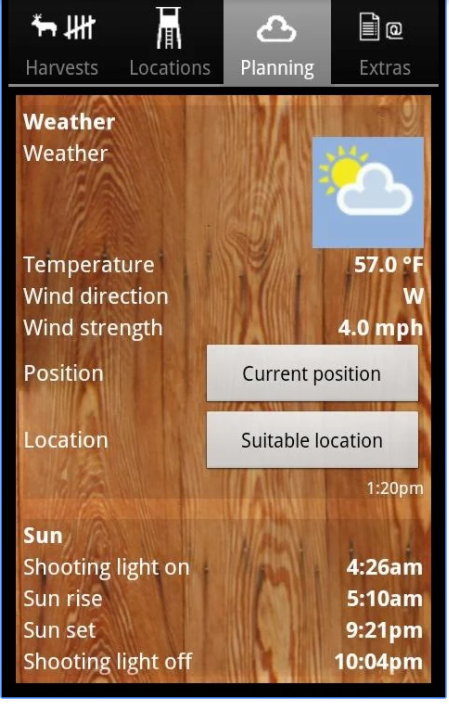
\includegraphics[width=6cm]{iHunt3.png}

\caption{Planificación con iHunt}
\label{fig:iHunt3}
\end{minipage}
\begin{minipage}[b]{0.5\linewidth}
\centering
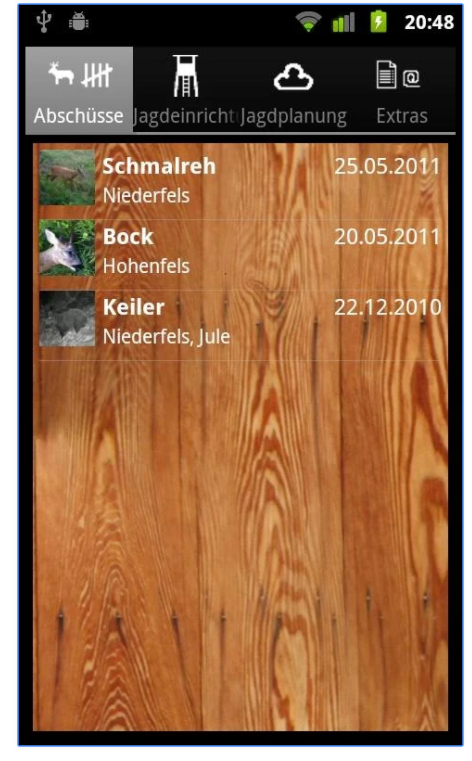
\includegraphics[width=6cm]{iHunt4.png}

\caption{Registro de trofeo con iHunt}
\label{fig:iHunt4}
\end{minipage}
\end{figure}

iHunt Journal está disponible desde iPhone y Android .


\subsection{My Fishing Companion}
 My Fishing Companion se trata de una aplicación para salir de pesca para Smartphone Android. Nos da la posibilidad de localizar nuestros lugares de capturas  véase figura \ref{fig:pesca2}, añadir vídeos y fotos, ver el tiempo que nos espera véase figura \ref{fig:pesca4},marcar capturas  véase figura \ref{fig:pesca3}, o las fases de la luna. También es interesante la comunidad en la que se comparten todos estos datos y que te pueden ayudar a elegir el mejor lugar y el mejor día de pesca.
 
 \begin{figure}[htbp]
\begin{minipage}[b]{0.5\linewidth} %Una minipágina que cubre la mitad de la página
\centering
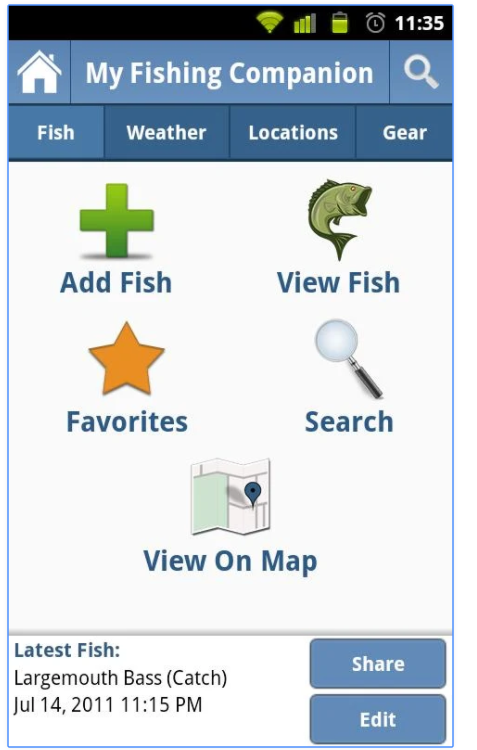
\includegraphics[width=6cm]{pesca1.png}
\caption{ Opciones de la aplicación}
\label{fig:pesca1}
\end{minipage}
\hspace{0.5cm} % Si queremos tener un poco de espacio entre las dos figuras
\begin{minipage}[b]{0.5\linewidth}
\centering
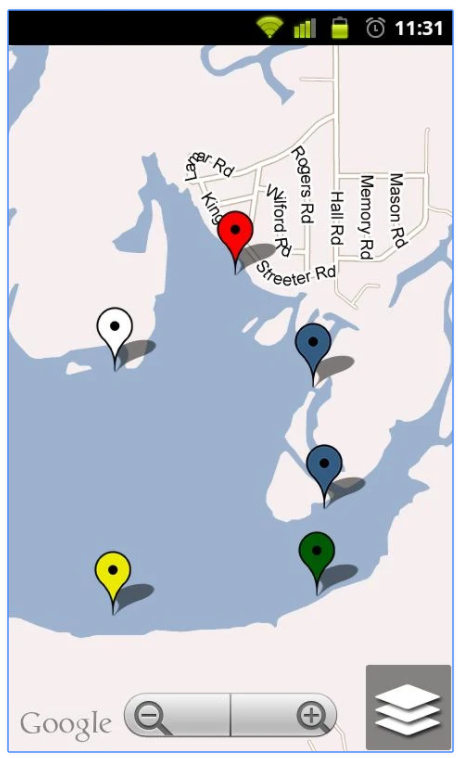
\includegraphics[width=6cm]{pesca2.png}

\caption{Puntos de pesca guardados}
\label{fig:pesca2}
\end{minipage}
\begin{minipage}[b]{0.5\linewidth}
\centering
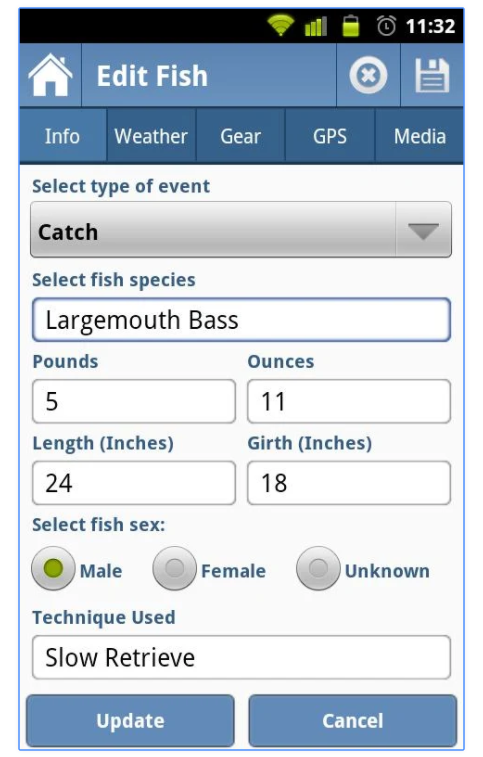
\includegraphics[width=6cm]{pesca3.png}

\caption{Datos de una captura}
\label{fig:pesca3}
\end{minipage}
\begin{minipage}[b]{0.5\linewidth}
\centering
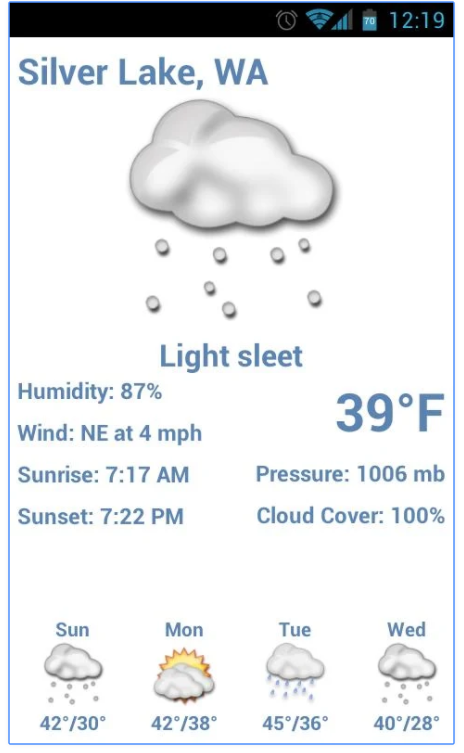
\includegraphics[width=6cm]{pesca4.png}

\caption{Datos sobre la meteorología}
\label{fig:pesca4}
\end{minipage}
\end{figure}